\documentclass[a4paper,10pt]{article}
\usepackage[utf8]{inputenc}
\usepackage{amsmath}
\usepackage{amsthm}
\usepackage{amsfonts}
\usepackage{amssymb}
\usepackage{fullpage}
\usepackage[german]{babel}
\setlength{\parindent}{0cm}
\usepackage{setspace}
\usepackage{mathpazo}
%\usepackage{cancel} % for strike through
\usepackage{graphicx}
\usepackage{wasysym} 
\usepackage{booktabs}
\usepackage{verbatim}
\usepackage{enumerate}
\usepackage{qtree}
\usepackage{ulem}
\usepackage{stmaryrd}
\usepackage{textcomp}
\usepackage[a4paper, left=1.8cm, right=1.8cm, top=2.0cm, bottom=2.0cm]{geometry}
\usepackage{tikz}
\usepackage{etex}
%\usepackage{algpseudocode} % For pseudo code
\usepackage{color}
\usetikzlibrary{calc, trees, petri,decorations,arrows,automata,shapes,shadows,positioning,plotmarks}
\pgfdeclarelayer{bg}    % declare background layer
\pgfsetlayers{bg,main}  % set the order of the layers (main is the standard layer)
\usepackage[arrow, matrix, curve]{xy}
\usepackage[shortlabels]{enumitem}

\newcommand{\N}{\mathbb{N}}
\newcommand{\A}{\mathcal{A}}
\newcommand{\R}{\mathbb{R}}
\newcommand{\C}{\mathbb{C}}
\newcommand{\Per}{\mathbb{P}}

\newcommand{\cd}{\cdot}
\newcommand{\tst}{\textstyle}
\newcommand{\lt}{\left}
\newcommand{\rt}{\right}
\newcommand{\ts}{\textsf}
\newcommand{\abs}[1]{\ensuremath{\left\vert#1\right\vert}}
\newcommand{\can}[1]{\langle #1 \rangle}
\newcommand{\hff}{~\text{\textit{ff}}}
\newcommand{\htt}{~\text{\textit{tt}}}
\newcommand{\must}[1]{[#1]}
\usepackage{tabularx}
\newcommand{\ddef}{\overset{def}=}
\newcommand{\wt}{~\text{\Aquarius}~}

\newcolumntype{L}[1]{>{\raggedright\arraybackslash}p{#1}}
\newcolumntype{C}[1]{>{\centering\arraybackslash}p{#1}}
\newcolumntype{R}[1]{>{\raggedleft\arraybackslash}p{#1}}

\begin{document}
\begin{center}
\Large{Cognitive Algorithms Assignment 6} \\
\end{center}
\begin{tabbing}
Tom Nick \hspace{2cm}\= - 340528\\
Maximilian Bachl \> - 341455 \\
\end{tabbing}

\section*{Aufgabe 2}
\section*{Aufgabe 3}
\section*{Aufgabe 4}

\subsection*{NMF}
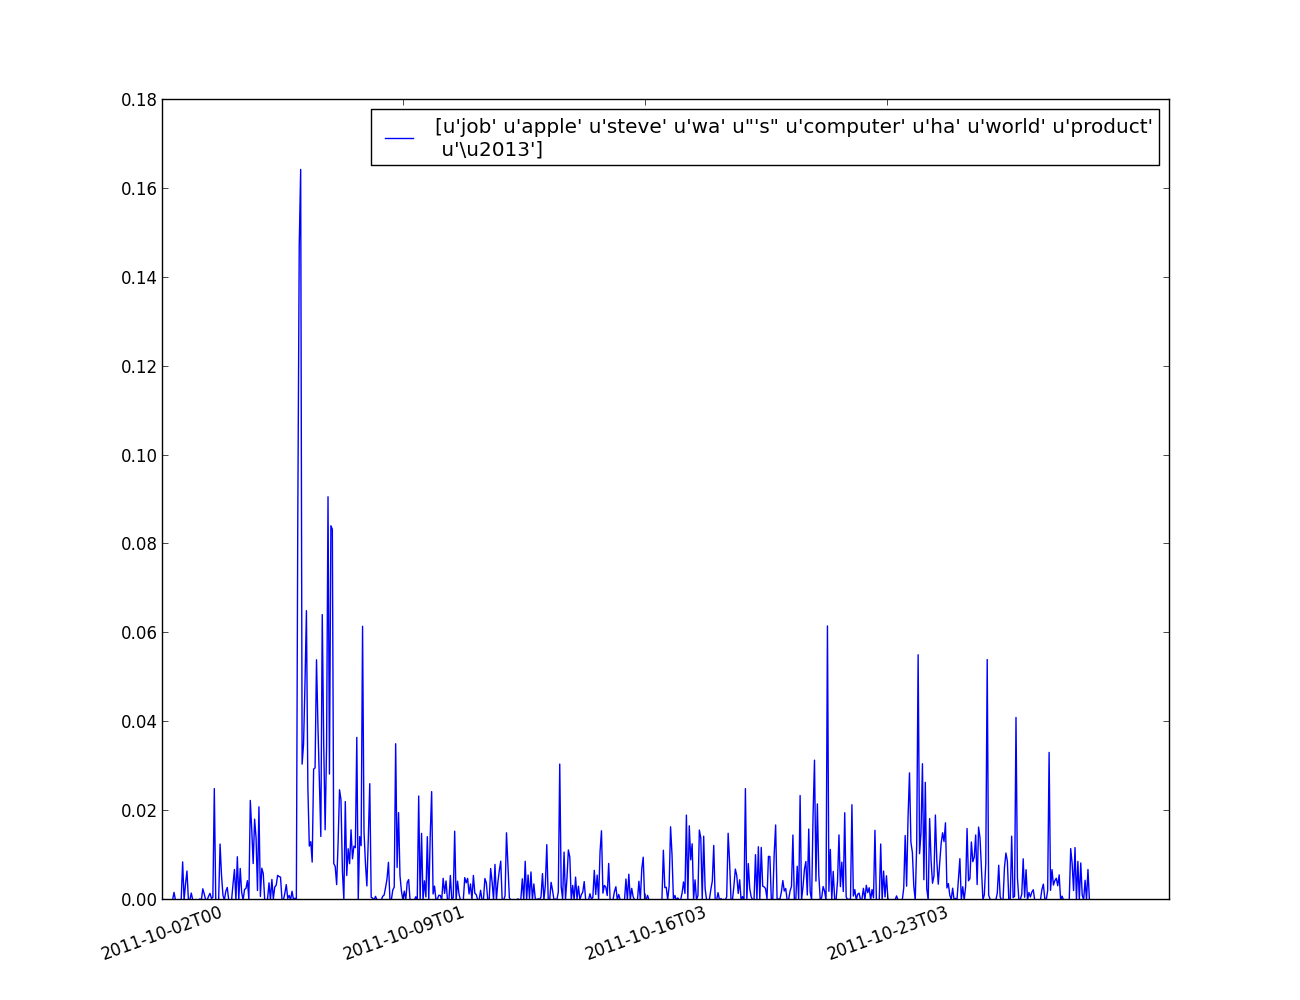
\includegraphics[width=20cm]{nmf_exercise_4.png}

\subsection*{PCA}
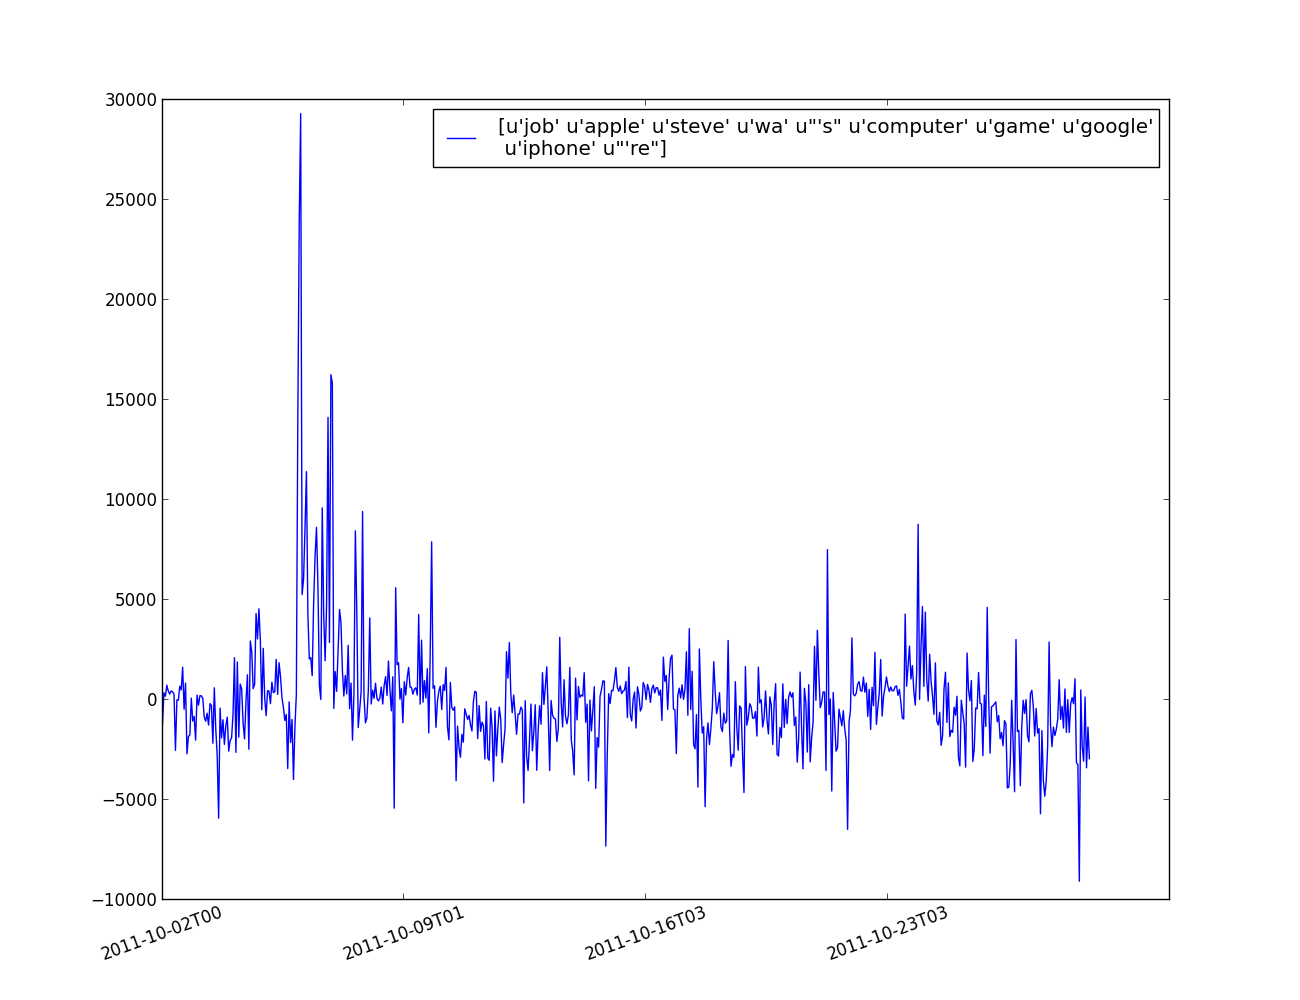
\includegraphics[width=20cm]{pca_exercise_4.png}

		
\end{document}








